\clearpage
\subsection{Standalone Desktop--Pi Clock-Offset Measurement}
\label{sec:standalone-desktop-pi}
The September 28 experiment isolates the Desktop--Pi part of the clock map. It compares a temporary wired Pi connection with the normal Pi Wi-Fi connection, without operating the motors or accessing Teensy. It measures clock offset and network round trip; it does not directly measure either one-way delay. All results in this subsection belong to this standalone session, not to the September 27 moving runs.

\subsubsection{Connections and Acquisition}
Figure~\ref{fig:desktop-pi-clock-network} shows the actual arrangement. Desktop remains wired to an ASUS LAN port, and an additional cable connects Pi to another ASUS LAN port. Pi Wi-Fi remains on AirBears 3. Desktop keeps its home-router Wi-Fi connection for Internet access. The Pi Ethernet address \texttt{10.0.0.24} was assigned by DHCP and may change; the existing Desktop \texttt{10.0.0.2} and Pi Wi-Fi \texttt{10.0.0.149} reservations remain in use. This is Ethernet through ASUS, not a direct Desktop--Pi cable.

\begin{figure}[H]
\centering
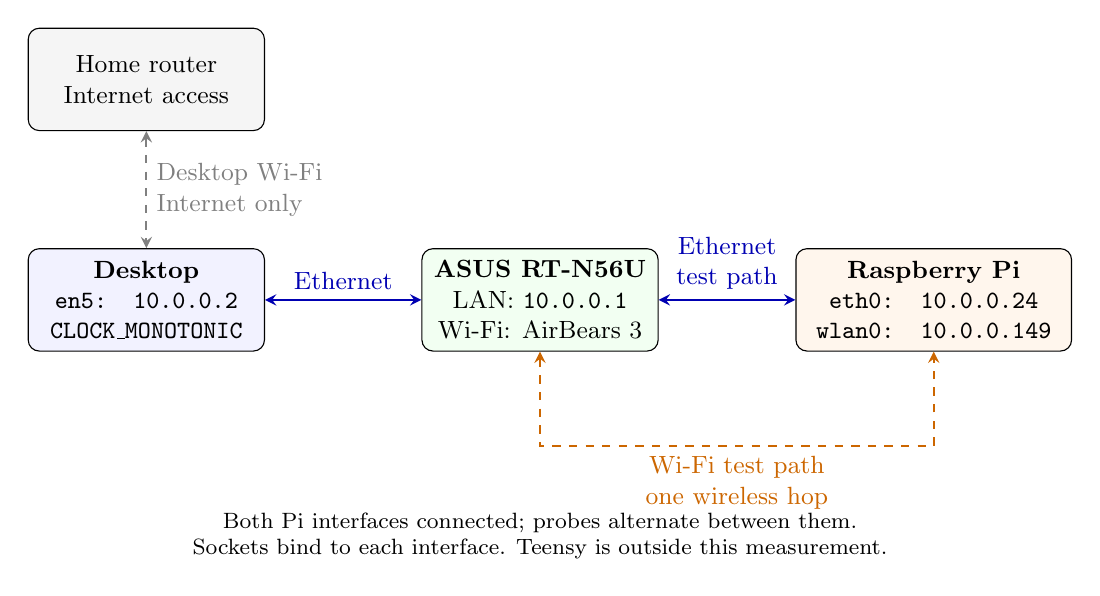
\begin{tikzpicture}[font=\small,box/.style={draw,rounded corners,align=center,minimum width=3cm,minimum height=1.3cm},link/.style={<->,thick,>=stealth}]
\node[box,fill=blue!5] (desktop) at (0,0) {\textbf{Desktop}\\\texttt{en5: 10.0.0.2}\\\texttt{CLOCK\_MONOTONIC}};
\node[box,fill=green!5] (asus) at (5,0) {\textbf{ASUS RT-N56U}\\LAN: \texttt{10.0.0.1}\\Wi-Fi: AirBears 3};
\node[box,fill=orange!7,minimum width=3.5cm] (pi) at (10,0) {\textbf{Raspberry Pi}\\\texttt{eth0: 10.0.0.24}\\\texttt{wlan0: 10.0.0.149}};
\node[box,fill=gray!8] (home) at (0,2.8) {Home router\\Internet access};
\draw[link,dashed,gray] (home) -- node[right,align=left] {Desktop Wi-Fi\\Internet only} (desktop);
\draw[link,blue!70!black] (desktop) -- node[above] {Ethernet} (asus);
\draw[link,blue!70!black] (asus.east) -- node[above,align=center] {Ethernet\\test path} (pi.west);
\draw[link,dashed,orange!80!black] (asus.south) -- ++(0,-1.2) -| node[pos=.25,below,align=center] {Wi-Fi test path\\one wireless hop} (pi.south);
\node[align=center,font=\footnotesize] at (5,-3.0) {Both Pi interfaces connected; probes alternate between them.\\Sockets bind to each interface. Teensy is outside this measurement.};
\end{tikzpicture}

\caption{Standalone clock-offset experiment. The wired and wireless Pi paths are measured separately while both remain connected. The Pi Ethernet link negotiated 100\,Mb/s full duplex. Desktop's home Wi-Fi carries Internet traffic, not the measurement probes.}
\label{fig:desktop-pi-clock-network}
\end{figure}

The standalone package is \path{2026_measure_pi_desktop_clock/} on Desktop, alongside the robot and operator packages. Its C++17 \texttt{clock\_probe} executable runs on both processors; Pi's copy is under \path{/home/pi/robot0/measure_pi_desktop_clock/}. Python launches the processes and analyzes saved data, outside the timestamp-critical path. C++ provides direct socket and timestamp-control access without an interpreter in the acquisition loop; it does not make either OS deterministic.

Two Pi UDP servers bind explicitly to \texttt{eth0} and \texttt{wlan0}, using ports 53120 and 53121. Desktop binds to \texttt{en5}. Incoming interface indices are checked, preventing a nominal Wi-Fi reply from silently taking Ethernet. Probes alternate between paths at approximately 20 probes/s/path, reversing pair order. Each request/reply application frame is 192 bytes, with session, probe and server-instance identifiers plus timestamps and diagnostics. This size differs from the robot's 82/36-byte SENSOR/COMMAND pair.

\subsubsection{Timestamp Method and Uncertainty}
For each exchange, $D_1$ is Desktop send time, $P_2$ Pi receive time, $P_3$ Pi reply time and $D_4$ Desktop receive time. Both receivers use kernel software receive timestamps. Desktop transmission is timestamped immediately before the application sends. Pi Ethernet uses a kernel software transmit timestamp matched by packet ID and returned in a follow-up datagram; $D_4$ still refers to the original reply. Pi's Wi-Fi driver does not advertise software transmit timestamping, so that path uses an application send timestamp. Thus the link comparison also includes different Pi transmit boundaries.

The Linux \href{https://docs.kernel.org/networking/timestamping.html}{socket timestamping interface} supplies receive/transmit metadata and packet IDs for matching transmit timestamps. Neither tested Pi interface exposes a hardware PTP clock; this experiment uses no NIC hardware timestamps. Kernel realtime timestamps are explicitly converted to each host's \texttt{CLOCK\_MONOTONIC} through nearby bracketed clock reads. Conversion and quantization allowances are retained in the uncertainty budget; clocks are never set or reset.

Here the displayed sign is $\psi=\text{Desktop}-\text{Pi}=-\phi$, giving positive values for this boot pair. Causality gives
\begin{equation}
 D_1-P_2\leq\psi\leq D_4-P_3,
 \qquad R_{DP}=(D_4-D_1)-(P_3-P_2).
\end{equation}
Pi turnaround is removed from the corrected round trip. The midpoint estimates offset; the half-width bounds the unknown directional asymmetry under the clock assumptions. The analysis expands each interval for timestamp mapping, quantization and an assumed 2000\,ppm rate guard across the probe. It does not divide latency equally between the two directions and call the result exact.

One-second window intersections additionally use a stated 50\,ppm rate allowance, with 2000\,ppm sensitivity results retained. A separate affine fit permits constant relative drift with at most 10\,$\mu$s model deviation over the run. These are conditional models, not verified oscillator specifications. A narrow histogram or a large sample count cannot remove an unknown fixed directional bias.

\subsubsection{Results and Interpretation}
The idle capture lasted 120\,s with 2400 probes per path; a second 60\,s capture used one busy C++ thread on Pi's single core and 1200 probes per path. All 7200 probes were valid, with no missing/rejected replies or Ethernet transmit-timestamp matching failures. Both runs used the same Pi boot ID. The load test represents CPU contention, not a full moving-robot workload.

\begin{table}[H]
\centering\small
\caption{Standalone Desktop--Pi results, September 28. All times are ms. The final column is the narrowest expanded individual-probe offset interval half-width, at that probe's instant; it is not a guaranteed uncertainty throughout a later job.}
\label{tab:standalone-desktop-pi}
\begin{tabular}{@{}llrrrr@{}}
\toprule
Condition & Pi link & Probes & RTT min. & RTT median & Best $\pm u$ \\
\midrule
Idle, 120 s & Ethernet & 2400 & 0.521 & 0.994 & 0.266 \\
Idle, 120 s & Wi-Fi & 2400 & 1.403 & 1.996 & 0.706 \\
CPU load, 60 s & Ethernet & 1200 & 0.504 & 0.971 & 0.257 \\
CPU load, 60 s & Wi-Fi & 1200 & 1.365 & 2.003 & 0.687 \\
\bottomrule
\end{tabular}

\end{table}

\begin{figure}[H]
\centering
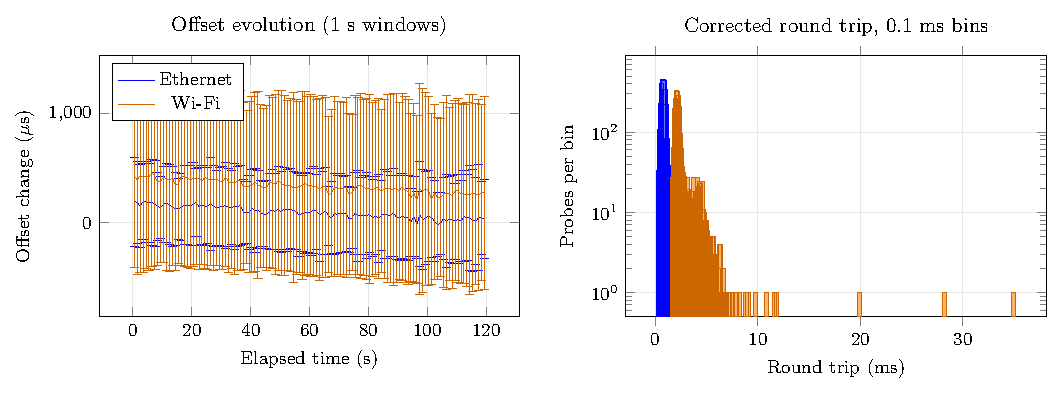
\includegraphics[width=\linewidth]{figures/pi_desktop_clock/20260928_073819_idle_plots.pdf}
\caption{Idle experiment: offset evolution and corrected round-trip distribution. The left panel subtracts one constant offset and plots one-second interval midpoints with conditional error bars using the 50\,ppm window assumption. The right panel includes all observed round trips in 0.1\,ms bins with logarithmic counts. Offset spread is not absolute accuracy.}
\label{fig:standalone-clock-results}
\end{figure}

Ethernet gave about $\pm0.26$--$\pm0.27$\,ms offset bounds, versus $\pm0.69$--$\pm0.71$\,ms over the Pi Wi-Fi path. The idle Ethernet affine estimate at elapsed 59.990\,s was Desktop minus Pi $=1118378.889885639$\,s $\pm0.270$\,ms under its model. The large positive value is the difference between clock origins, not a network delay. Sub-0.1\,ms absolute accuracy has not been demonstrated. The observed Ethernet median RTT was about 1\,ms, versus about 2\,ms on Wi-Fi; these are round trips of the standalone probes, not motor-control cycles.

Combining a fresh wired bound with the assumed 0.1\,ms GPIO allowance suggests a Desktop--Teensy uncertainty floor of roughly $\pm0.36$--$\pm0.37$\,ms before extrapolation, fitting and other mapping allowances. This is a prospective budget, not a measured integrated result. A cable removal does not itself reset the monotonic clocks, but subsequent drift needs a validated holdover model; 1\,ppm rate error alone accumulates 0.06\,ms per minute. No untethered holdover test was performed. A reboot invalidates the old calibration. These measurements cannot be retroactively applied to the earlier robot runs or interpreted as a reduction in their physical communication delay.

\begin{sloppypar}
Raw integer-nanosecond timestamps, reports and plots are in the standalone package's \path{out/20260928_073819_idle/} and \path{out/20260928_074049_cpu_load/}. The latest analyzed summary is \path{out/desktop_pi_clock.latest.json}. \texttt{run\_measurement.py} launches acquisition; \texttt{analyze.py} and \texttt{affine\_bounds.py} produce the intervals and plots. This report's copied figures, source hashes and derived tables are under \path{docs/figures/pi_desktop_clock/}; reproduce the tables with \path{docs/tools/report_pi_desktop_clock.py}.
\end{sloppypar}
